\section{Large language models (LLMs)}

\subsection{Introduction}

Language modeling is a long-standing research topic, dating back to the 1950s with Shnnon's application of information theory to human language, where he measures how well simple n-gram language models predict or compress natural language text \cite{6773263}. Since then, statistical language modeling became fundamental to many natural language understanding and generation tasks, ranging from speech recognition, machine translation, to information retrieval \cite{Jelinek1997StatisticalMF} \cite{Manning_Raghavan_Schütze_2008}.

Recent advances in transformer-based large language models (LLMs), pretrained on web-scale text corpora, have significantly enhanced the capabilities of these models. For instance, OpenAI's ChatGPT and GPT-4 are now used not only for natural language processing but also as general task solvers, exemplified by their integration into Microsoft's Co-Pilot systems. These models can follow complex human instructions and perform multi-step reasoning when necessary. Consequently, LLMs are becoming fundamental building blocks for the development of general-purpose AI agents or artificial general intelligence (AGI).

LLMs are large-scale, pre-trained, statistical language models based on neural networks. Their recent success is the result of decades of research and development in language modeling, which can be divided into four distinct waves, each with its own starting points and progression: statistical language models, neural language models, pre-trained language models, and LLMs.

Early neural language models (NLMs) \cite{NIPS2000_728f206c}, \cite{schwenk-etal-2006-continuous}, \cite{mikolov10_interspeech}, \cite{graves2014generating} address data sparsity by mapping words to low-dimensional continuous vectors, known as embedding vectors, and predicting the next word based on the aggregation of these vectors using neural networks. The embedding vectors learned by NLMs create a hidden space where the semantic similarity between vectors can be easily computed as their distance. This enables the computation of semantic similarity between any two inputs, regardless of their forms (e.g., queries versus documents in web search \cite{10.1145/2505515.2505665}, \cite{gao2022neural}, sentences in different languages in machine translation \cite{sutskever2014sequence}, \cite{cho2014properties}) or modalities (e.g., image and text in image captioning \cite{cho2014properties}, \cite{vinyals2015tell}). However, early NLMs are task-specific models, as they are trained on task-specific data, resulting in a hidden space that is also task-specific.

Pre-trained language models (PLMs), unlike early neural language models (NLMs), are task-agnostic. This generality also extends to the learned hidden embedding space. The training and inference of PLMs follow the pre-training and fine-tuning paradigm, where language models utilizing recurrent neural networks \cite{peters2018deep} or transformers \cite{devlin2019bert}, \cite{liu2019roberta}, \cite{he2021deberta} are pre-trained on web-scale unlabeled text corpora for general tasks such as word prediction. They are then fine-tuned for specific tasks using small amounts of labeled, task-specific data. Recent surveys on PLMs include \cite{zhou2023comprehensive}, \cite{han2021pretrained}, \cite{Qiu_2020}.

Large language models (LLMs) mainly refer to transformer-based neural language models that contain tens to hundreds of billions of parameters. These models, such as PaLM \cite{chowdhery2022palm}, LLaMA \cite{touvron2023llama}, and GPT-4 \cite{openai2024gpt4}, are pre-trained on massive text datasets. Compared to pre-trained language models (PLMs), LLMs are not only significantly larger in model size but also exhibit stronger language understanding and generation abilities. More importantly, they demonstrate emergent abilities not present in smaller-scale language models. As illustrated in Figure \ref{fig:llm-capabilities}, these emergent abilities include:

\textbf{In-context learning}: LLMs can learn a new task from a small set of examples presented in the prompt at inference time.

\textbf{Instruction following}: After instruction tuning, LLMs can follow instructions for new types of tasks without explicit examples.

\textbf{Multi-step reasoning}: LLMs can solve complex tasks by breaking them down into intermediate reasoning steps, as demonstrated in the chain-of-thought prompting \cite{wei2023chainofthought}.

LLMs can also be augmented with external knowledge and tools \cite{mialon2023augmented}, \cite{mialon2023augmented}, enabling them to effectively interact with users and the environment \cite{mialon2023augmented}, and continually improve using feedback data collected through interactions, such as via reinforcement learning with human feedback (RLHF).

\begin{figure}[H]
    \centering
    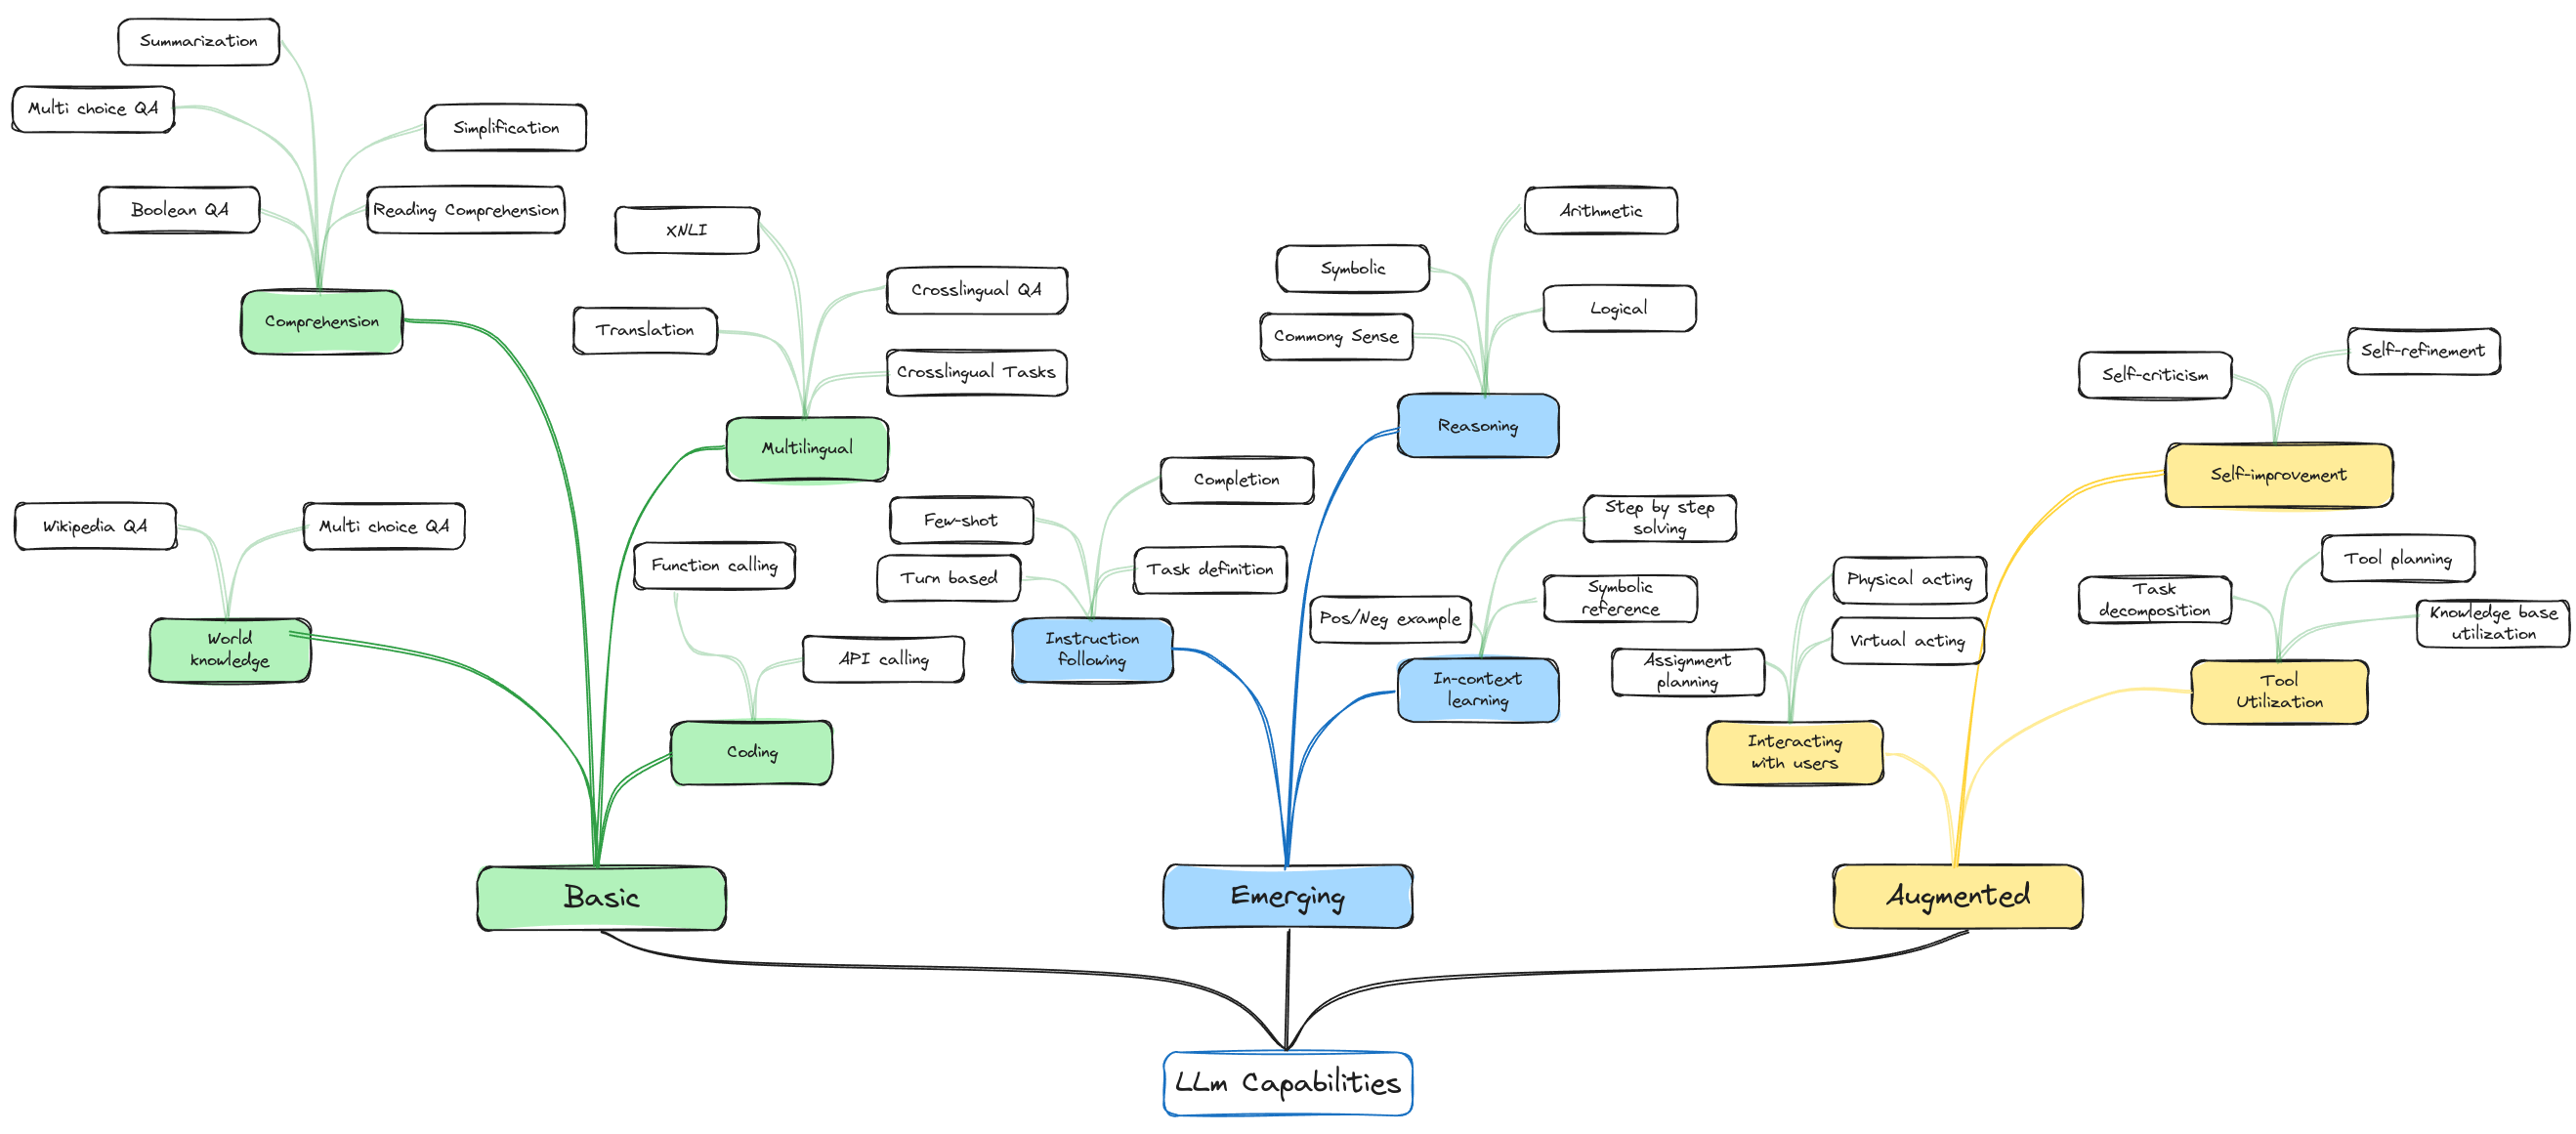
\includegraphics[width=\textwidth,height=6cm,keepaspectratio=true]{llm-capabilities.png}
    \caption{
        \it{LLM capabilities \cite{minaee2024large}}
    }
    \label{fig:llm-capabilities}
\end{figure}

\subsection{Large Language Model Families}

Large language models (LLMs) primarily refer to transformer-based pre-trained language models (PLMs) that encompass tens to hundreds of billions of parameters. Compared to the previously discussed PLMs, LLMs are significantly larger in size and demonstrate enhanced capabilities in language understanding, generation, and emergent phenomena that are absent in smaller models. This section will examine three prominent LLM families: GPT, LLaMA, and PaLM, as illustrated in Figure \ref{fig:llm-families}

\begin{figure}[H]
    \centering
    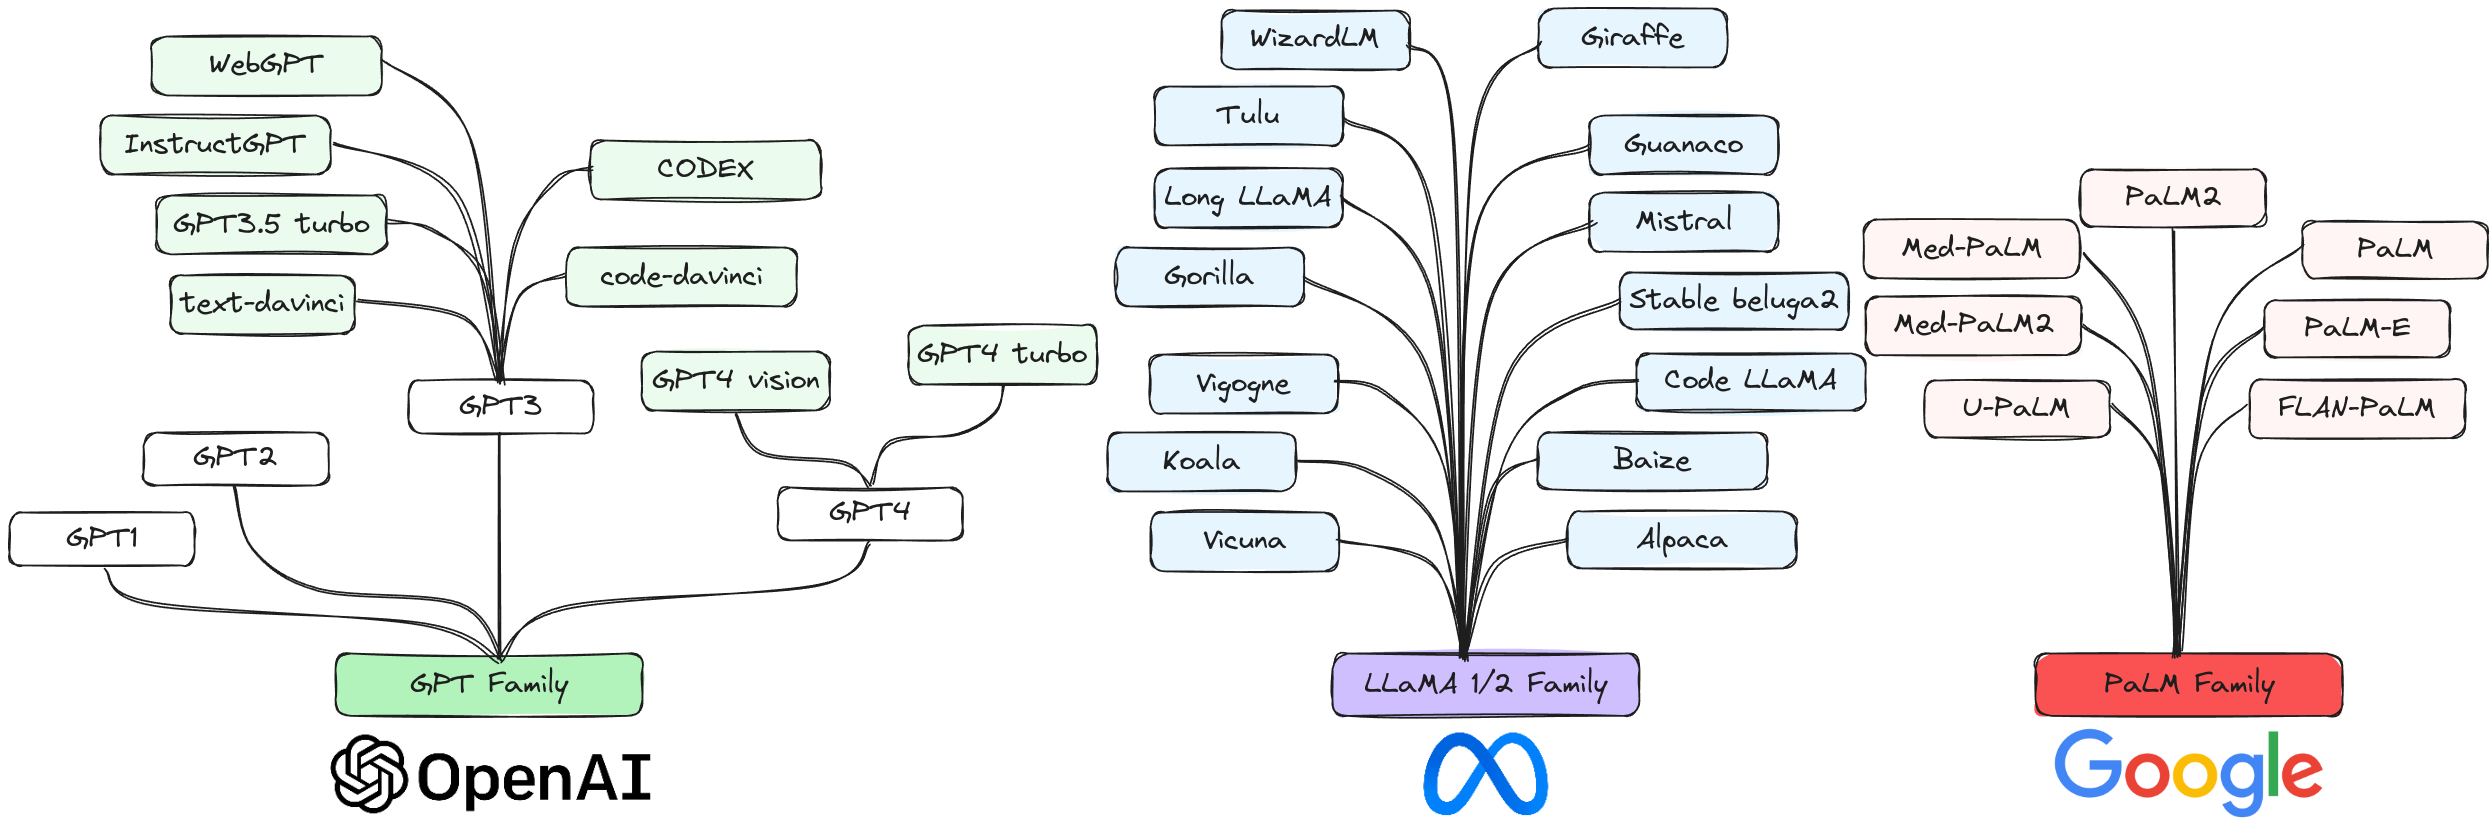
\includegraphics[width=\textwidth,height=6cm,keepaspectratio=true]{llm-families.png}
    \caption{
        \it{Popular LLM families \cite{minaee2024large}}
    }
    \label{fig:llm-families}
\end{figure}